% Valentino Vranic
% Metody inzinierskej prace 2012/13

\documentclass{beamer}

%\usetheme{Warsaw}
%\usetheme{Antibes}
\usetheme{JuanLesPins}
%\usetheme{Goettingen}

%\usecolortheme{seahorse}
%\usecolortheme{dolphin}
\usecolortheme{rose}
% http://deic.uab.es/~iblanes/beamer_gallery/index_by_color.html
%\usecolortheme{beaver}

%\useoutertheme[]{sidebar}

\setbeamercovered{transparent}

\usepackage[slovak]{babel}
\usepackage[T1]{fontenc}
\usepackage[utf8]{inputenc}
\usepackage{url}

\usepackage{listings}

\lstset{language=C++,basicstyle=\fontsize{8}{9.6}\selectfont,showstringspaces=false,columns=fullflexible,identifierstyle=\ttfamily,keywordstyle=\bfseries,showstringspaces=false,columns=fullflexible}
%\lstset{language=C,basicstyle=\fontsize{10.5}{12.6}\selectfont,identifierstyle=\ttfamily,keywordstyle=\bfseries,showstringspaces=false,columns=fixed}

\def\BibTeX{\textsc{Bib}\kern-.08em\TeX} 

\newcommand{\footcite}[1]{\footnote{\tiny #1}}
\newcommand{\umlet}{.5}
\newcommand{\emp}[1]{\textit{\alert{#1}}}
\newcommand{\kw}[1]{\mbox{\textbf{#1}}}
\newcommand{\id}[1]{\texttt{#1}}
\newcommand{\stl}{\guillemotleft}
\newcommand{\str}{\guillemotright}

\newcommand{\lsti}{\lstinline[basicstyle=\fontsize{10.5}{12.1}\selectfont]}

\newcommand{\ssection}[1]{
	\section{#1}
	\begin{frame}[fragile=singleslide]\frametitle{}
	\Huge #1
	\end{frame}
}

\newcommand{\ssectionn}[1]{
	\section*{#1}
	\begin{frame}[fragile=singleslide]\frametitle{}
	\Huge #1
	\end{frame}
}

\newenvironment{program}{\begin{beamercolorbox}[rounded=true,shadow=true]{block body}\vspace{-4mm}}{\vspace{-2mm}\end{beamercolorbox}}

\setbeamercolor{fvystup}{fg=white,bg=black}
\newenvironment{vystup}{\begin{beamercolorbox}[rounded=true,shadow=true]{fvystup}}{\end{beamercolorbox}}

\newenvironment{poznamka}{\begin{beamercolorbox}[rounded=true,shadow=false]{block body}}{\end{beamercolorbox}}

\setbeamertemplate{footline}[page number]
{
%\insertpagenumber
%\begin{beamercolorbox}{section in head/foot}
%\vskip2pt\insertnavigation{\paperwidth}\vskip2pt
%\end{beamercolorbox}%
}



\author{Dávid Zachar}
%\url{www.fiit.stuba.sk/~vranic}, \url{vranic@fiit.stuba.sk}}
%{\tiny \url{www.fiit.stuba.sk/~vranic}, \url{vranic@fiit.stuba.sk}}
\institute{
	Faculty of Informatics and Information Technologies\\
	Sllovak University of Technology in Bratislava}

\subtitle{\vspace{3mm} Engineering Methods 2022/2023}

\title{The benefits of playing video games
}

\date{\footnotesize 22. november 2022}




\begin{document}

\begin{frame}[fragile=singleslide]
\titlepage
\end{frame}


\begin{frame}[fragile=singleslide]\frametitle{Introduction to the topic}
\begin{itemize}
	\item Video games are getting more and more popular
	\item Amount of hours spent playing video games is rising too
	\item We start to question whether video games have some positive effects
\end{itemize}
\end{frame}


\begin{frame}[fragile=singleslide]\frametitle{Contents}
\tableofcontents
\end{frame}


%\section{Graph}
% príkaz \ssection by vytvoril zvláštný slajd s názvom časti - v krátkych prezentáciách to prekáža, lebo oberá o čas

\begin{frame}[fragile=singleslide]\frametitle{The graph will be here}
\begin{figure}
	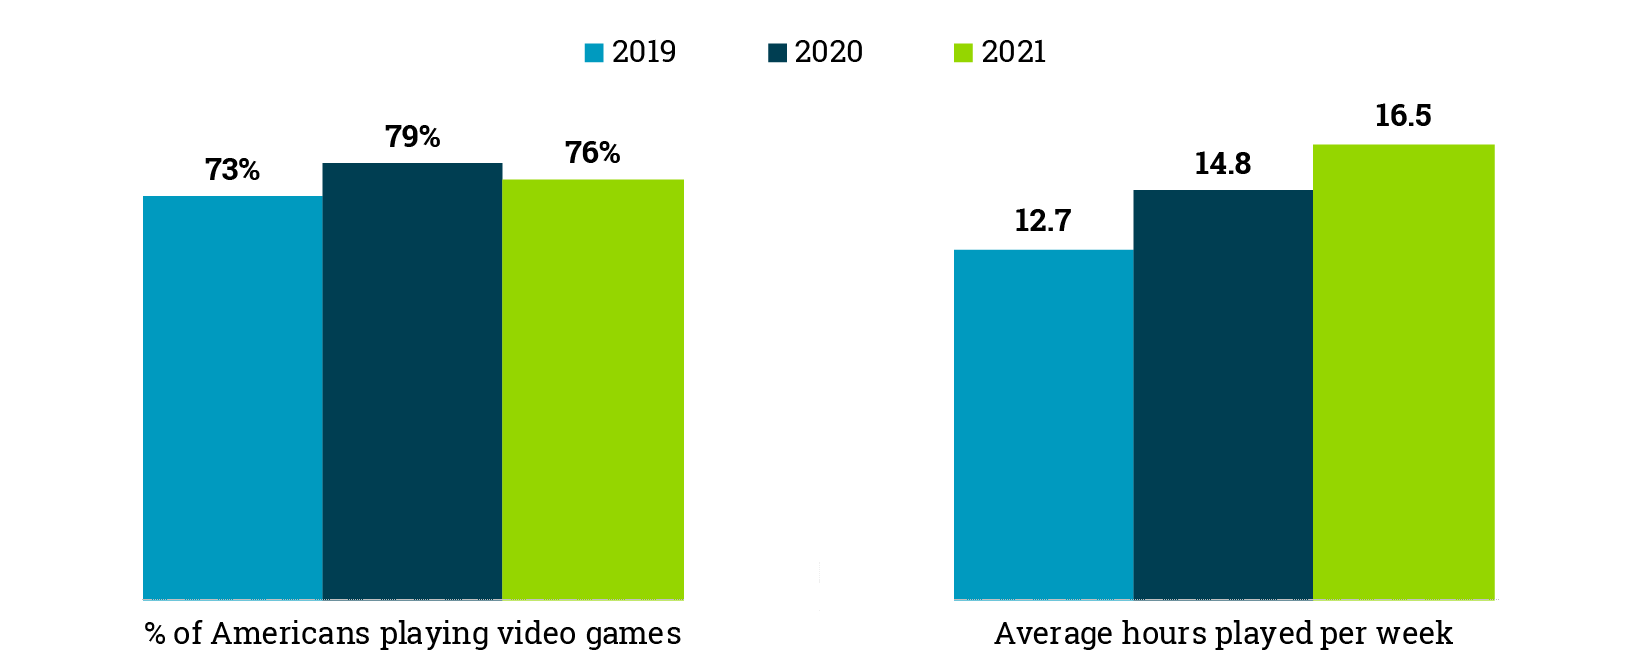
\includegraphics[scale=.35]{graf1.png}
	{\tiny Video games playing trends}
\end{figure}
\end{frame}



%\section{Table will go here}

\begin{frame}[fragile=singleslide]\frametitle{Table}
\begin{itemize}
\item Nejaký text
\item Ďalší text -- \emph{zvýraznený text}
\item \emp{Kľúčová poznámka} % príkaz definovaný v preambule

% odrážka s odkazom na zdroj:
\item Bol použitý balík beamer\footcite{\url{http://www.tex.ac.uk/tex-archive/macros/latex/contrib/beamer/doc/beameruserguide.pdf}}
\end{itemize}
\end{frame}


\begin{frame}[fragile=singleslide]\frametitle{A slide with an image}
\begin{center}
	
\includegraphics[scale=.15]{POSTER.pdf}
	{\tiny This is a poster for my article}
\end{center}
% pridajte vlastný obrázok a zrušte znák % pred príkazom \includegraphics vo formáte PDF prípadne PNG alebo JPG
% scale určuje veľkosť obrázku


\end{frame}

\begin{frame}[fragile=singleslide]\frametitle{Methodology}
\begin{itemize}
	\item Video games are getting more and more popular
	\item Amount of hours spent playing video games is rising too
	\item We start to question whether video games have some positive effects
\end{itemize}
\end{frame}

\begin{frame}[fragile=singleslide]\frametitle{Literature review}
\begin{itemize}
	\item Video games are getting more and more popular
	\item Amount of hours spent playing video games is rising too
	\item We start to question whether video games have some positive effects
\end{itemize}
\end{frame}

%\section*{Summary}
% hviezdička zabezpečí, aby sa táto časť neocitla v prehľade prezentácie - každá prezentácia má zhodnotenie a prehľad by sa tým zbytočne zahlcoval

\begin{frame}[fragile=singleslide]\frametitle{Conclusion}
\begin{itemize}
\item Conclussin
\item Playing benefits can have its benefits as well as its negatives
\item As with everything things are not only black and white
\end{itemize}
\end{frame}


\end{document}




Text \end{document} za príkazom \end{document} LaTeX ignoruje, takže tu môžete odkladať veci (aj celé slajdy), ktoré nechcete vymazať, lebo ich ešte možno budete potrebovať, avšak ich v danom momente nechcete mať v slajdoch.
